\documentclass[14pt]{extarticle}
% math symbols
\usepackage{sfg}


\usepackage{amssymb,amsmath}
\synctex=1
% for different compilers
\usepackage{ifpdf}
% geometry of page
\usepackage[margin=2cm]{geometry}

% if pdflatex, then
\ifpdf
\usepackage[russian]{babel}
\usepackage[utf8]{inputenc}
\usepackage[unicode]{hyperref}
\usepackage[pdftex]{graphicx}
\usepackage{cmlgc}
% if xelatex, then
\else
% math fonts
\usepackage{fouriernc}
% xelatex specific packages
\usepackage[xetex]{hyperref}
\usepackage{xltxtra}	% \XeLaTeX macro
\usepackage{xunicode}	% some extra unicode support
\defaultfontfeatures{Mapping=tex-text}
\usepackage{polyglossia}	% instead of babel in xelatex
\usepackage{indentfirst}	% 
\setdefaultlanguage{russian}
% fonts
\newfontfamily\cyrillicfont{SchoolBookC}
\newfontfamily\cyrillicfontsf{TextBookC}
\setmonofont{Consolas}
\fi

% several pictures in one figure
\usepackage{subfig}
% calc in TeX expressions
\usepackage{calc}
% nice pictures and plots
\usepackage{pgfplots,tikz,circuitikz}
% different libraries for pictures
\usetikzlibrary{%
  arrows,%
  calc,%
  patterns,%
  decorations.pathreplacing,%
  decorations.pathmorphing,%
  decorations.markings,%
  intersections,%
  decorations.text%
}

\usepackage{tkz-euclide}

\usepackage{enumitem}
\renewcommand{\theenumi}{(\asbuk{enumi})}
\renewcommand{\labelenumi}{\asbuk{enumi})}
\AddEnumerateCounter{\Asbuk}{\@Asbuk}{\CYRM}
\AddEnumerateCounter{\asbuk}{\@asbuk}{\cyrm}

\begin{document}

\section*{Задача}

\subsection*{Условие}
Точки $A$ и $B$ лежат в двух перпендикулярных плоскостях вне их общей прямой. Сколько существует точек $X$ на их общей прямой, таких что треугольник $AXB$ прямоугольный?
\subsection*{Решение}
Пусть $H_b$ -- проекция точки $B$ на $m$. Аналогично $H_a$ -- проекция точки $A$ на $m$. Найдем все решения. Пусть на $m$ есть такая точка $X$, что $(\overrightarrow{AX}, \overrightarrow{XB})=0$.

Если ввести на $m$ координату, то это будет квадратным уравнением. То есть больше двух корней быть не может. Обнаружим эти корни.

Есть 2 решения $X=H_a, H_b$, поскольку $AX\perp XB$ по свойству перпендикуляра к плоскости.
\newpage
\begin{figure}[h]
	\centering
	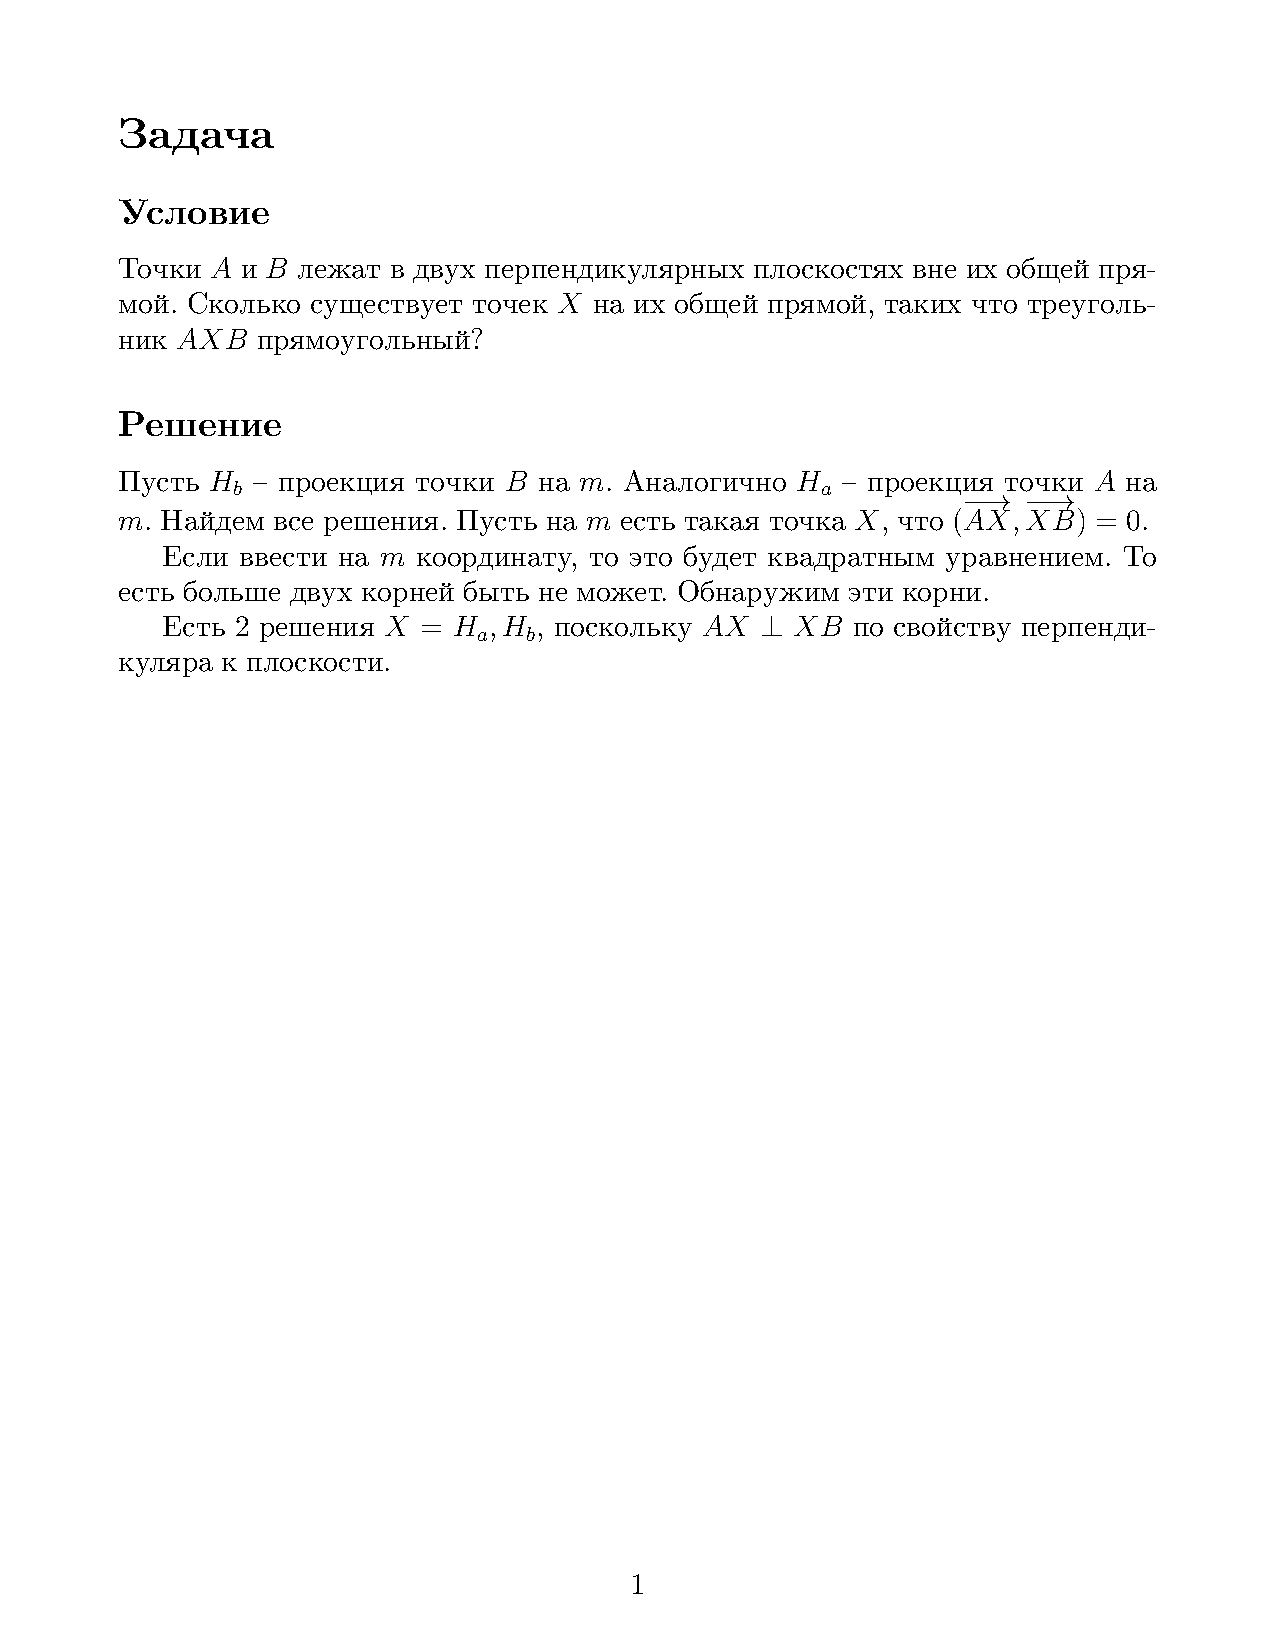
\includegraphics[width=1\textwidth]{{/home/galqiwi/geoma/8.4}.png}
\end{figure}


\end{document}